\subsection{Implementation}
%
Der Ablauf der Kalibrierung ist in Abbildung~\ref{fig:calibration_flowchart} in Form eine Ablaufdiagramms dargestellt. Beschrieben werden die wesentlichen Schritte. Es sind sowohl Interaktion mit der Person enthalten, die die Kalibrierung durchführt, als auch die Schritte, die von den beteiligten Softwarekomponenten ausgeführt werden enthalten. Es wurden im Rahmen der Arbeit zwei unterschiedliche Wege implementiert, um ein Ergebnis für die Kalibrierung zu berechnen. Diese Wege werden im Folgenden vorgestellt und die Ergebnisse miteinander verglichen. Die Präsentation der Resultate wird vor allem dazu verwendet werden, die gewählte Form der Diagramme zu erläutern. Diese werden in den Ergebnissen des komplexeren Modells ebenfalls verwendet.
%
\subsubsection{SVD}
%
Das unter \ref{sec:svd} vorgestellte Verfahren der Singular-Value-Decomposition kann dazu verwendet werden eine Lösung eines linearen Gleichungssystems zu berechnen. Das Modell, das zur Kalibrierung verwendet wird, ist ein Gleichungssystem der Form $\mathbf{A}\mathbf{x}=\mathbf{b}$ und hat drei Gleichungen mit drei Unbekannten. Daher kann sofort eine Lösung mit dem Verfahren hergeleitet werden. Das Ergebnis eines Messaufbaus mit 3 Antennen ist in Tabelle~\ref{tab:FinalCoords} und in Abbildung~\ref{fig:3dplot_coordinates} gezeigt. Die Implementation des Algorithmus stammt aus \cite{press2007numerical} und wurde für diese Arbeit angeschafft.
%
\subsubsection{CMA-ES}
Da in dieser Arbeit der CMA-ES-Algorithmus eingesetzt wird und damit ohnehin eine Implementation vorgenommen wird, kann die Kalibrierung dazu verwendet werden die Umsetzung des Algorithmus zu verifizieren. Dazu vergleichen wir die Lösung der SVD-Methode mit der des CMA-ES.\\
Das über den evolutionären Algorithmus gefundene Ergebnis gleicht dem des SVD-Verfahrens (siehe Tabelle~\ref{tab:FinalCoords}). Der SVD-Algorithmus ist um ein vielfaches effizienter\footnote{d.h. weniger Rechenzeit ist erforderlich} beim Lösen des Gleichungssystems. Die Gründe, warum an dieser Stelle die Berechnung mit dem evolutionären Verfahren durchgeführt und hier dargestellt wird sind folgende:
%
\begin{enumerate}
 \item Die Komplexität ist gering, daher kann der Ablauf des evolutionären Verfahrens besser dargestellt und verstanden werden
 \item Der Vergleich der beiden Ergebnisse ermöglicht die Verifizierung der Implementation beider Verfahren.
\end{enumerate}
%
Dem ersten Punkt kommt im Rahmen dieser Arbeit eine besondere Stellung zu. Es ist einfacher anhand dieses übersichtlichen Problems (mit nur drei Unbekannten) den Ablauf des Algorithmus sowie die Visualisierung der Ergebnisse zu veranschaulichen. Die verwendete Darstellung gleicht der, die später bei der Präsentation und Beurteilung der komplexeren Modell verwendet wird. Die Ergebnisse werden in dem Kapitel~\ref{sec:calibrationResults} gezeigt.
%
%
\begin{figure}[ht!]
         \centering
         \caption[Kalibrierwerkzeuge]{Werkzeuge, die bei der Kalibrierung verwendet werden.}
         \begin{subfigure}[t]{0.4\textwidth}
                 \centering
                 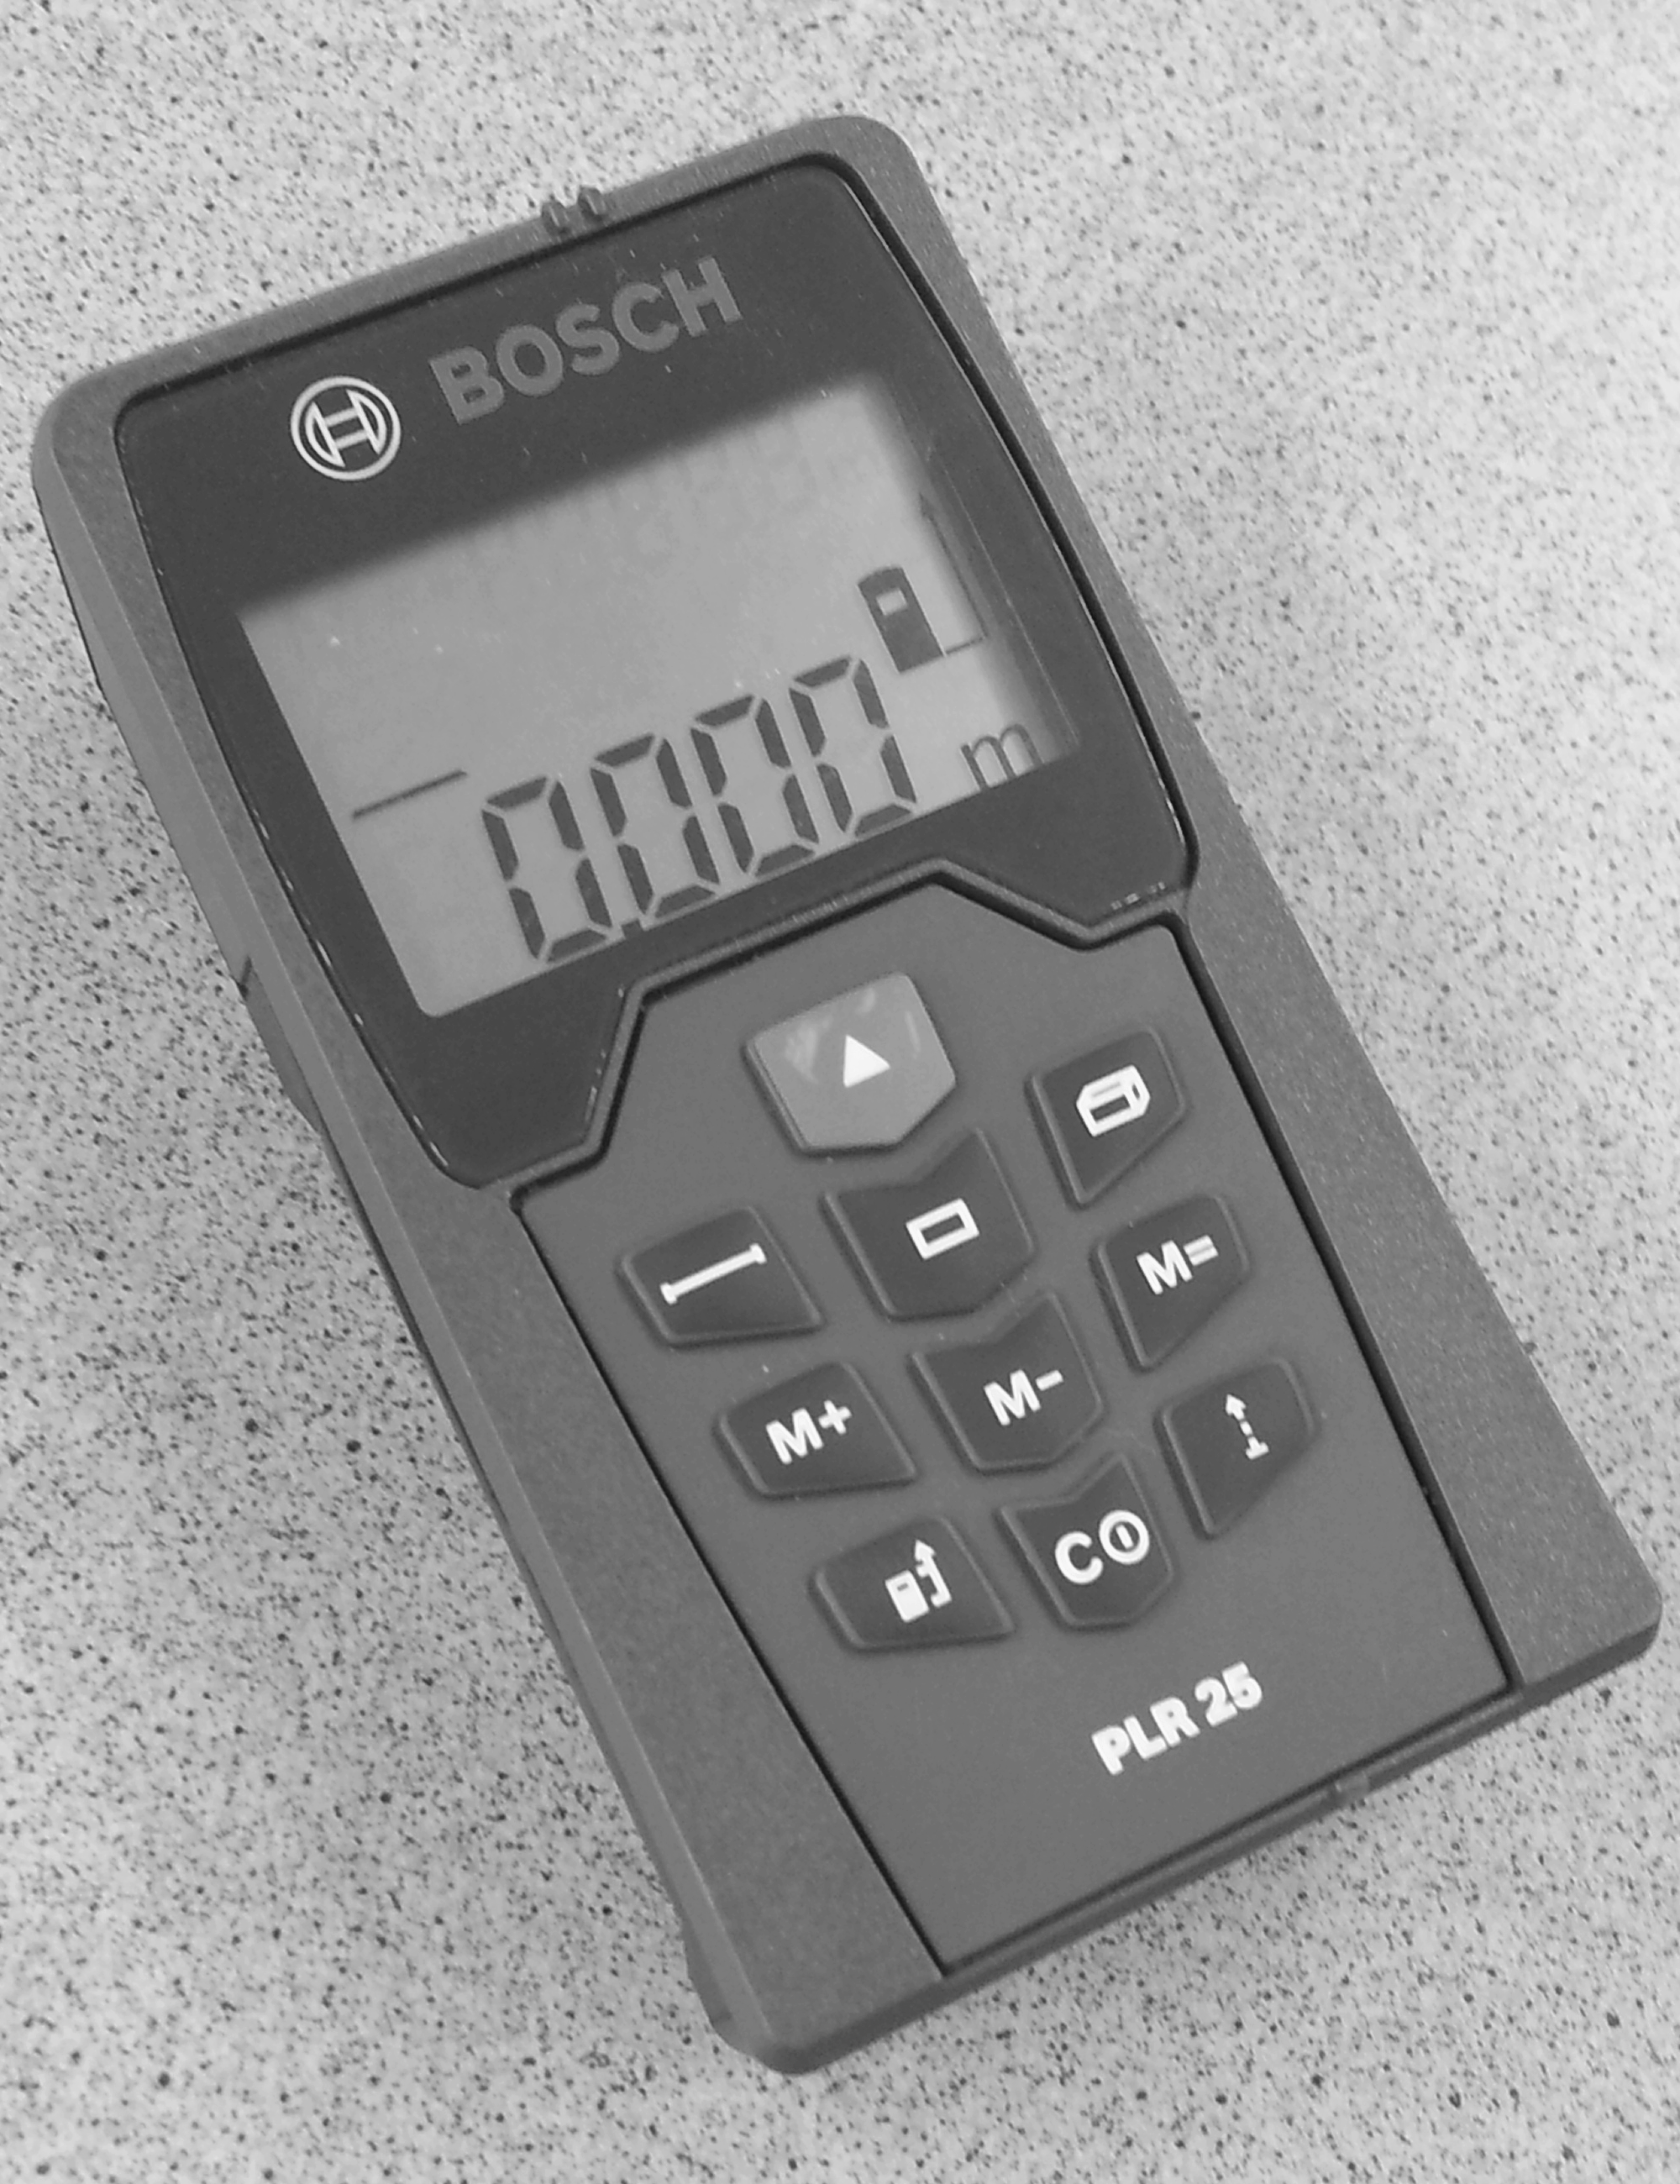
\includegraphics[width=\textwidth]{img/Lasermeter.png}
                 \caption{Laser Distanzmesser}
                 \label{fig:laser_meter}
         \end{subfigure}
%
\qquad         
%
         \begin{subfigure}[t]{0.4\textwidth}
                 \centering
                 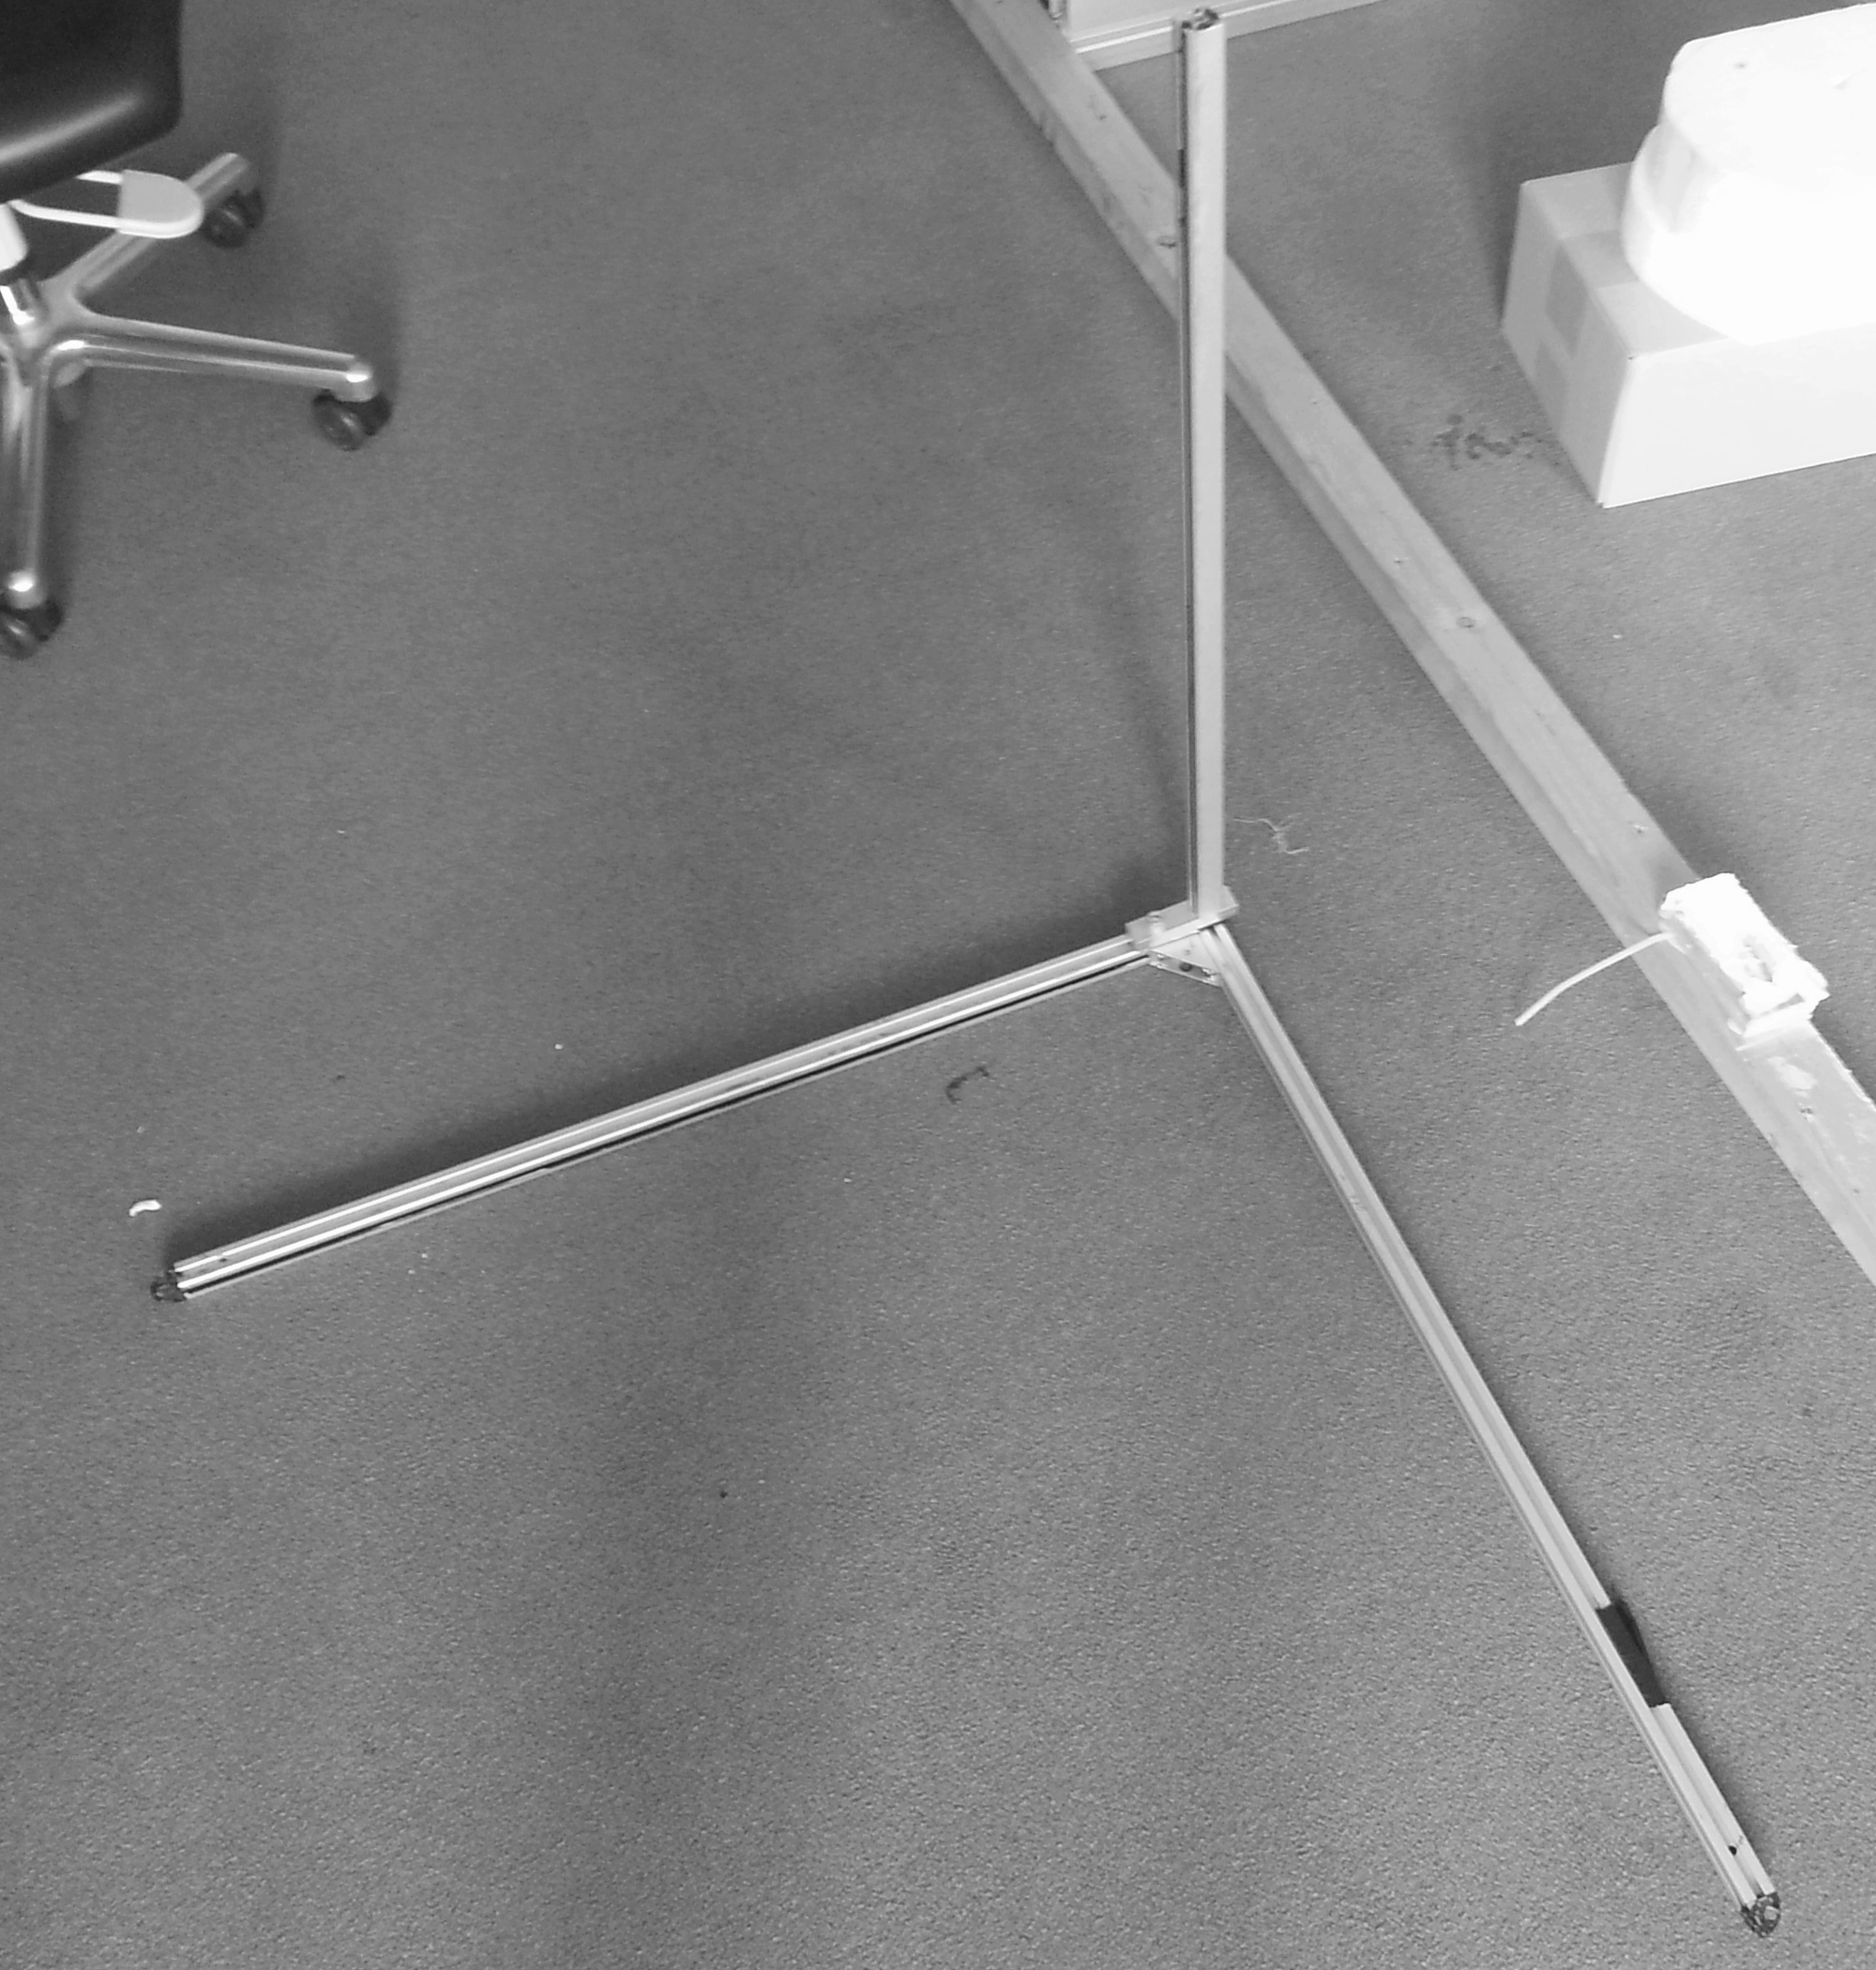
\includegraphics[width=\textwidth]{img/Calibration_Phantom.png}
                 \caption{Kalibrierstück mit vier Messpositionen. }
                 \label{fig:calib_piece}
         \end{subfigure}
         \label{fig:Calibration_Tools}
\end{figure}
%
%-------------------------------------------------------------------------
\begin{figure}[H]
	\begin{center}
		\caption[Ablauf der Kalibierung]{Ablauf der Kalibierung}
		\label{fig:calibration_flowchart}
		\vspace{0.5cm}
		\begin{tikzpicture}[auto]
		\scriptsize
			\tikzstyle{decision} = [diamond, draw=black, thick, fill=black!20, text width=5em, text badly centered, inner sep=1pt]
%			
			\tikzstyle{block} = [rectangle, draw=black, thick, fill=gray!20, text width=15em, text centered, rounded corners, minimum height=4em]
%	
			\tikzstyle{line} = [draw, thick, -latex',shorten >=1pt];
			\tikzstyle{commentline} = [draw, dashed, green!50,-latex',shorten >=1pt];
%	
			\tikzstyle{cloud} = [ dotted, draw=green!50, thick, ellipse,,fill=green!20, minimum height=2em, text width= 10em, text badly centered];
%	
			\matrix [column sep=5mm,row sep=7mm]
			{
				% row 1
				& \node [block] (start) { Start }; & \\
				% row 2
				& \node [block] (setup) {Aufstellen des Kalibrierstücks}; & 
					\node [cloud] (comment1) {Gezeigt in Abbildung \ref{fig:calib_piece}}; \\
				% row 4
				& \node [block] (measure) {Vermessen der Entfernungen zu den Antennen}; & 
					\node [cloud] (comment2) {z.B. mit Laser-Entfernungsmesser, gezeigt in Abbildung \ref{fig:laser_meter}}; \\
				% row 5
				&\node [block] (writefile) {Eintragen der Vermessenen Werte in Mashinenlesbare Datei}; &\\
				% row 6
				\node (temp){}; &\node [block] (startsw) {Starte die Kalibiersoftware}; &\\
				% row 7
				&\node [block] (viewresults) {Speichern der berechneten Werte}; &\\
				% row 8				
				& \node [decision] (decide) {$\Delta \geq \Delta_{max}$}; & 
					\node [cloud] (criteria) {Ergebnisse haben eine geringe Abweichung};\\
				% row 9
				& \node [block] (stop) {Ende}; & \\
			};
			
%
%			Draw the arrows
%
			\path (decide) -| node [near start] {Nein} (temp);
			\tikzstyle{every path}=[line]
			\path (start) -- (setup);
			\path (setup) -- (measure);
			\path (measure) -- (writefile);
			\path (writefile) -- (startsw);
			\path (startsw) -- (viewresults);
			\path (viewresults) -- (decide);
			\path (decide)	-| +(-3,0)  |- (measure);
			\path (decide) -- node [midway] {Ja} (stop);
			
%			
%			draw the comments 
%
			\tikzstyle{every path}=[commentline]
			\path (criteria) -- (decide);
			\path (comment1) -- (setup);
			\path (comment2) -- (measure);
				
		\end{tikzpicture}
	\end{center}
\end{figure}
%
%-------------------------------------------------------------------------
\begin{figure}[ht!]
	\begin{center}
		\caption[Ablauf der libCalibration]{Ablauf der libCalibration}
		\label{fig:calibration_flowchart_}
		\vspace{1cm}
		\begin{tikzpicture}[auto]
		\scriptsize
			\tikzstyle{decision} = [diamond, draw=black, thick, fill=black!20, text width=5em, text badly centered, inner sep=1pt]
%			
			\tikzstyle{block} = [rectangle, draw=black, thick, fill=gray!20, text width=15em, text centered, rounded corners, minimum height=4em]
%	
			\tikzstyle{line} = [draw, thick, -latex',shorten >=1pt];
			\tikzstyle{commentline} = [draw, dashed, green!50,-latex',shorten >=1pt];
%	
			\tikzstyle{cloud} = [ dotted, draw=green!50, thick, ellipse,,fill=green!20, minimum height=2em, text width= 10em, text badly centered];
%	
			\matrix [column sep=5mm,row sep=7mm]
			{
				% row 1
				& \node [block] (start) { Start }; & \\
				% row 2
				& \node [block] (read) {Lese gemessene Werte aus CSV-Datei}; &  \\
				% row 4
				& \node [block] (read2) {Lade Geometrie des Kalibrierstücks}; & 
				 \node [cloud] (comment1) {Diagonalmatrix};\\
				% row 5
				&\node [block] (calc1) { Berechne die Matrizen für jede Antenne $\mathbf{A_k}\qquad,1 \leq k \leq |N|$ }; &  \\
				% row 6
				&\node [block] (calc2) { Berechne den Distanzvektor $\mathbf{b}$ }; &  \\			 
				% row 7
				&\node [block] (run) {Berechne die Positionen}; &
 				 \node [cloud] (comment2) {mittels SVD};\\
				% row 8
				&\node [block] (write) {Schreibe Werte}; &\\
				% row 9				
				& \node [block] (stop) {Ende}; & \\
			};
			
%
%			Draw the arrows
%
			\tikzstyle{every path}=[line]
			\path (start) -- (read);
			\path (read) -- (read2);
			\path (read2) -- (calc1);
			\path (calc1) -- (calc2);
			\path (calc2) -- (run);
			\path (run) -- (write);
			\path (write) -- (stop);
%			
%			draw the comments 
%
			\tikzstyle{every path}=[commentline]
			\path (comment1) -- (read2);
			\path (comment2) -- (run);
				
		\end{tikzpicture}
	\end{center}
\end{figure}
%\newpage
%
 